% Compiler: LaTeX => PDF

\documentclass{beamer}

\usepackage[ngerman]{babel}
\usepackage[utf8]{inputenc}

%\usepackage{multimedia}
\usepackage{graphicx}
\usepackage[nolist]{acronym}

\usepackage{stackengine}
\usepackage{array}

\usepackage{enumitem}

\setitemize{label=\usebeamerfont*{itemize item}%
  \usebeamercolor[fg]{itemize item}
  \usebeamertemplate{itemize item}}

\title{Streifenprojektion}
%\subtitle{X $\in \{$ Motion, Shading, Texture $\}$}
%\subtitle{Schwerpunkte: Shape from Motion, \\ Shape from Shading, Shape from Texture}
\author{Dennis Wagner, \\ Johannes Spangenberg, \\ Leroy Kramer}
%\date{\today}
\date{12.02.2014}

% add page number
\setbeamertemplate{footline}[frame number]

\begin{document}


\frame{\titlepage} 


\begin{frame}
	\frametitle{Gliederung}
	\tableofcontents
\end{frame} 


\section{0 \hspace{5px} Unsere Aufgabe} 
\begin{frame}
	\frametitle{Streifenprojektion}
	\framesubtitle{Unsere Aufgabe}
	[foto gesamt]
	
\end{frame}

% ---------------------------------------------------------------------------- %

\section{1 \hspace{5px} Umsetzung} 
\subsection{1.1 \hspace{5px} Hardware}
\begin{frame}
	\frametitle{Streifenprojektion}
	\framesubtitle{Hardware}
	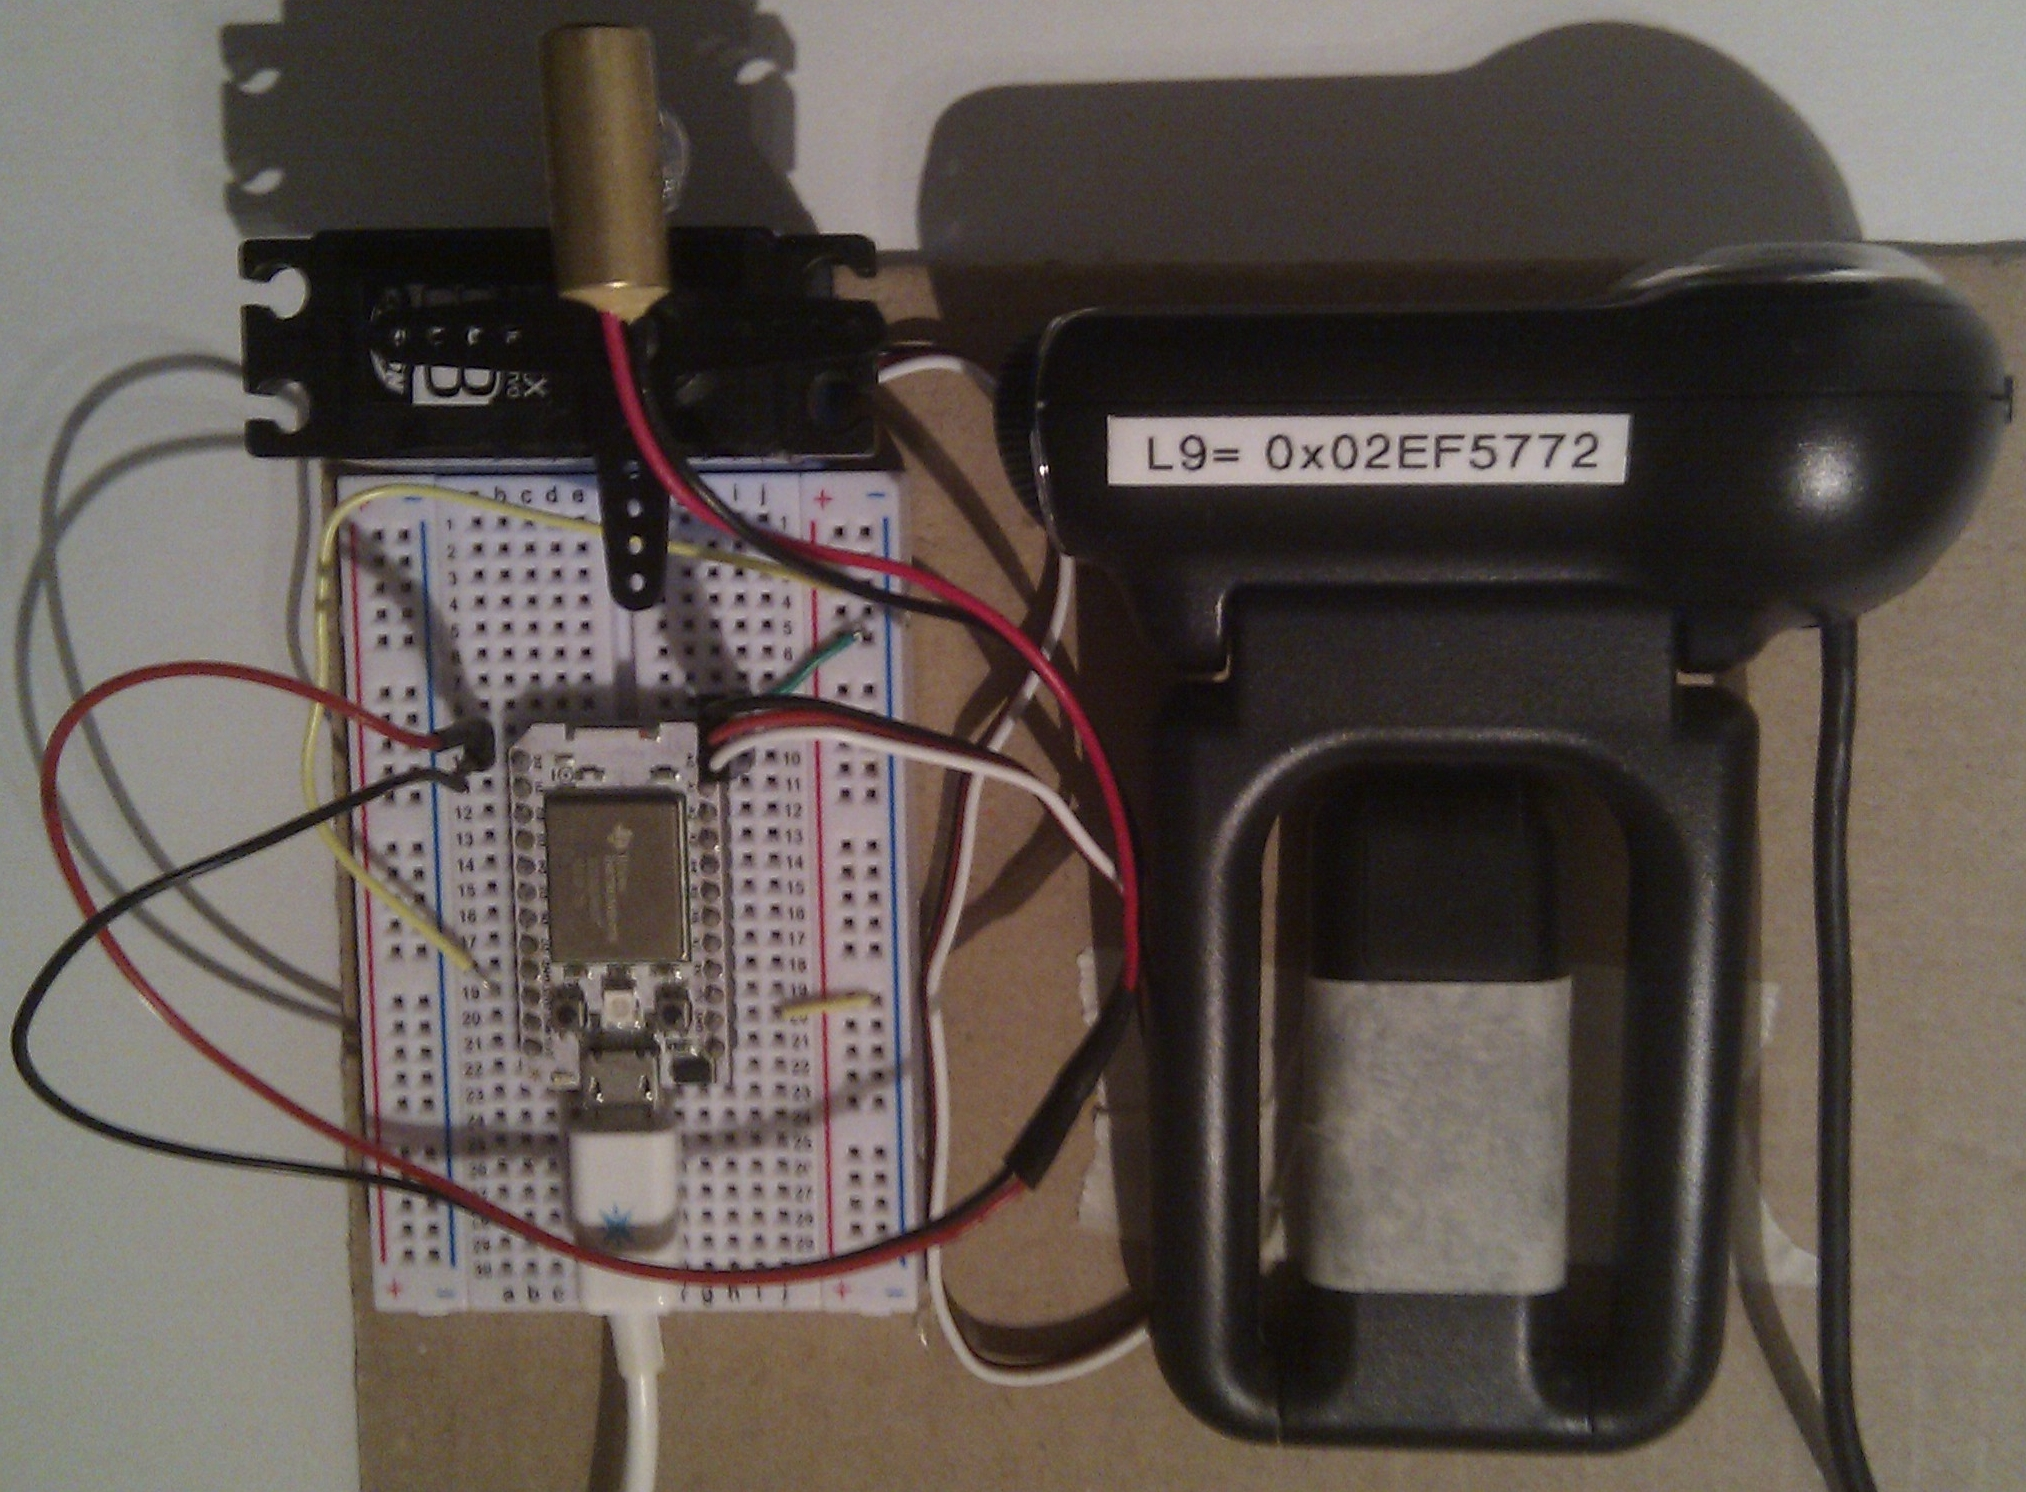
\includegraphics[width=\linewidth]{includes/hardware.jpg}
	
\end{frame}


\subsection{1.1 \hspace{5px} Software}
\begin{frame}
	\frametitle{Streifenprojektion}
	\framesubtitle{Software}
	[blockbild]
	
\end{frame}


\section{2 \hspace{5px} Live-Demo} 
\begin{frame}
	\frametitle{Streifenprojektion}
	\framesubtitle{Live-Demo}
	
\end{frame}


\section{3 \hspace{5px} Probleme} 
\begin{frame}
	\frametitle{Streifenprojektion}
	\framesubtitle{Probleme}
	[organisatiorischen]
	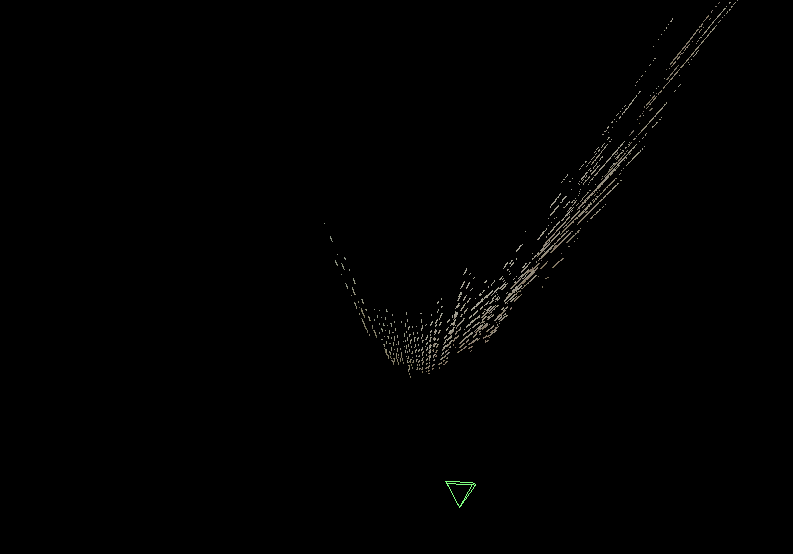
\includegraphics[width=\linewidth]{includes/krumm.png}
	[linien erkennung]
	[hardware aufbau]
	
	
\end{frame}

\section{4 \hspace{5px} Quellen} 
\begin{frame}
	\frametitle{Streifenprojektion}
	\framesubtitle{Quellen}
	
\end{frame}


\end{document}
